\documentclass[tikz]{standalone}
\usepackage{helvet}
\usepackage[T1]{sansmath}
\renewcommand{\familydefault}{\sfdefault}
\normalfont

\begin{document}
\begin{sansmath}

\tikzstyle{tallunit} = [
    draw, minimum height = 2cm, minimum width = 2cm, fill=blue!05,
    rectangle, rounded corners, text centered]

\tikzstyle{unit} = [
    draw, minimum height = 1cm, minimum width = 2cm, fill=blue!05,
    rectangle, rounded corners, text centered]

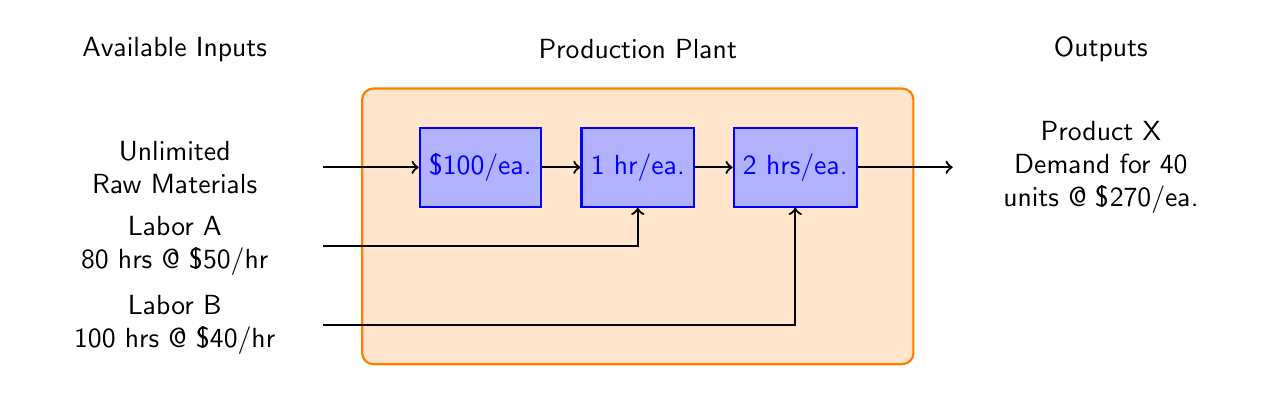
\begin{tikzpicture}[auto,thick]
    %\draw[help lines] (-1,1) grid (14,6);
    
    \draw [orange, fill=orange!20, rounded corners]
        (3,1.5) rectangle ++(7,3.5);
    \node [rectangle, blue, fill=blue!30, minimum width = 1cm, minimum height = 1cm, draw] 
        (box1) at (4.5,4) {\$100/ea.};
    \node [rectangle, blue, fill=blue!30, minimum width = 1cm, minimum height = 1cm, draw] 
        (box2) at (6.5,4) {1 hr/ea.};
    \node [rectangle, blue, fill=blue!30, minimum width = 1cm, minimum height = 1cm, draw] 
        (box3) at (8.5,4) {2 hrs/ea.};
        
    \draw (box1) ++(-2,1.5) 
        node [left,rectangle,align=center, text width = 3.5cm] {Available Inputs};
    \draw [<-] (box1) -- ++(-2,0) 
        node [left,rectangle, align=center, text width = 3.5cm]
        {Unlimited\\Raw Materials};
    \draw [<-] (box2) -- ++(0,-1) -- ++(-4,0) 
        node [left,rectangle, align=center, text width = 3.5cm] 
        {Labor A \\ 80 hrs @ \$50/hr};
    \draw [<-] (box3) -- ++(0,-2) -- ++(-6,0) 
        node [left,rectangle, align=center, text width = 3.5cm]
        {Labor B \\ 100 hrs @ \$40/hr};
    \draw [->] (box1) -- ++(box2);
    \draw [->] (box2) -- ++(box3);
    \draw [->] (box3) -- ++(2,0) 
        node [right,rectangle, align=center, text width = 3.5cm] 
        {Product X \\ Demand for 40 units @ \$270/ea.};
    \draw (box3) ++(2,1.5) 
        node [right,rectangle, align=center, text width = 3.5cm] {Outputs};
    
    \draw (6.5,5.5) node {Production Plant};
    
\end{tikzpicture}

\end{sansmath}
\end{document}
